\documentclass[compress]{beamer}



%

\usepackage[T1]{fontenc}
%\usepackage{kmath,kerkis}
%\usepackage{fouriernc}
\usepackage[adobe-utopia]{mathdesign}
%\usepackage{arev}
\usepackage{times}
\usepackage{natbib}

\usepackage[noend]{algpseudocode}
\usepackage{xmpmulti}
\usepackage{dsfont}
\usepackage{amsmath}

\usepackage{graphicx,float,wrapfig, bbm}
\usepackage{amsfonts, comment, bbold}
\usepackage{mdwlist}
\usepackage{subfigure}
\usepackage{colortbl}
\usepackage{mathrsfs}


\usepackage{multirow}




% packages

\usepackage{amsfonts}

% environments

\newenvironment{packed_enumerate}{
  \begin{enumerate}
    \setlength{\topsep}{0pt}
    \setlength{\itemsep}{2pt}
    \setlength{\parskip}{0pt}
    \setlength{\parsep}{0pt}
}{\end{enumerate}}

\newenvironment{stepit}
 {\begin{itemize}[<+-|alert@+>]}
   {\end{itemize}}

% commands

\newcommand{\Norm}[3]{\mathcal{N}\left( #1, #2, #3 \right)}
\newcommand{\popshow}[2]{\only<#1->{\alert<#1>{#2}}}
\newcommand{\x}{\mathbf{x}}
\newcommand{\ex}[1]{\mbox{exp}\left\{ #1\right\} }
\newcommand{\e}[2]{\mathbb{E}_{#1}\left[ #2 \right] }
\newcommand{\g}{\, | \,}
\newcommand{\indpt}{\protect\mathpalette{\protect\independenT}{\perp}}
\def\independenT#1#2{\mathrel{\rlap{$#1#2$}\mkern2mu{#1#2}}}
\newcommand{\E}{\textrm{E}}
\newcommand{\R}{\textrm{R}}
\newcommand{\realline}{\mathbb{R}}
\newcommand{\data}{{\cal D}}
\newcommand{\loglik}{{\cal L}}
\newcommand{\grad}[2]{ \frac{\partial{#1}}{\partial#2}}
\newcommand{\dir}[1]{\mbox{Dir}(#1)}
\newcommand{\mult}[1]{\mbox{Mult}( #1)}
\newcommand{\G}[1]{\Gamma \left( \textstyle #1 \right)}
\newcommand{\ind}[1]{\mathds{1}\left[ #1 \right] }
\newcommand{\norm}[1]{\left\lVert#1\right\rVert}

\newcommand{\class}[1]{ \texttt{#1}}
\newcommand{\term}[1]{ ``#1''}
\newcommand{\tcword}[0]{ w }
\newcommand{\docsetlabeled}[0]{ D }
\newcommand{\onedoclabeled}[0]{ d }
\newcommand{\tcposindex}[0]{ i }
\newcommand{\myblue}[1]{ {\textbf #1 }}
\newcommand{\dnrm}[1]{ _{\mbox{\textsc{ #1 }}}}
\newcommand{\argmax}[0]{ \arg \max }
\newcommand{\tcjclass}[0]{c_j}
\newcommand{\maths}[1]{ {\bf #1}}




% complexity
\renewcommand{\O}{\mathcal{O}}



\setbeamersize{text margin left=0.5cm}
\setbeamersize{text margin right=0.5cm}
\setbeamercolor{alert}{fg=red!75!black}

\usetheme{default}
\useinnertheme{circles}
\useoutertheme{split}
\usecolortheme{seahorse}
% \usecolortheme{dove}
% \usecolortheme{seagull}
%\usecolortheme{default}
% \usecolortheme{dolphin}
\usefonttheme{structurebold}
%\usefonttheme{serif}

\setbeamertemplate{navigation symbols}{}
\setbeamertemplate{headline}{}
\setbeamertemplate{footline}{}
\setbeamerfont{itemize/enumerate subbody}{size=\normalsize}
\setbeamerfont{itemize/enumerate subsubbody}{size=\normalsize}
\setbeamercolor{itemize item}{fg=gray}
\setbeamercolor{enumerate item}{fg=gray}
\setbeamercolor{itemize item}{fg=gray}
\setbeamercolor{itemize subitem}{fg=gray}
\setbeamercolor{item projected}{bg=gray}
\setbeamercolor{subitem projected}{bg=gray}


\newenvironment{bullets}
{\begin{itemize} \setlength{\itemsep}{10pt}}
{\end{itemize}}

\newcommand{\mygraphic}[2]{
  \begin{beamercolorbox}[colorsep*=4pt]{black math}
    \begin{center}
      \includegraphics[#1]{#2}
    \end{center}
  \end{beamercolorbox}
}

\setbeamercolor{structure}{bg=gray}
\setbeamercolor{section in head/foot}{bg=gray}
\setbeamercolor{palette primary}{bg=lightgray}


\usepackage{minted}

\usetheme[pageofpages=of,                    % String used between the current page and the
                                             % total page count.
          bullet=circle,                     % Use circles instead of squares for bullets.
          titleline=true,                    % Show a line below the frame title.
          showdate=true,                     % show the date on the title page
          alternativetitlepage=true,         % Use the fancy title page.
          titlepagelogo=../../common/culogo,              % Logo for the first page.
          % Logo for the header on first page.
          headerlogo=../../common/boulder_cs,
          ]{UCBoulder}

\usecolortheme{ucdblack}
\author{Introduction to Data Science Algorithms}


\institute[Boyd-Graber and Paul] % (optional, but mostly needed)
{Jordan Boyd-Graber and Michael Paul}


\AtBeginSection[] % "Beamer, do the following at the start of every section"
{ \begin{frame} \frametitle{Outline} % make a frame titled "Outline"
\tableofcontents[currentsection] % show TOC and highlight current section
\end{frame} }


\usepackage{tikz-dependency}
%\usepackage{tikz-qtree}
\usepackage{qtree}
\usepackage{pdfpages}

\newcommand{\gfx}[2]{
\begin{center}
	\includegraphics[width=#2\linewidth]{distsim/#1}
\end{center}
}
\title{Distributional Semantics}
\date{Slides Adapted from Yoav Goldberg and Omer Levy}

\begin{document}

\tikzstyle{every picture}+=[remember picture]



\begin{frame}
  \titlepage
\end{frame}


\begin{frame}{Beyond word2vec}

    \begin{itemize}
        \item word2vec is factorizing a word-context matrix.
        \item The content of this matrix affects the resulting similarities.
        \item word2vec allows you to specify a \textit{window size}.
        \item But what about other types of contexts?
    \end{itemize}

    \begin{itemize}
        \item Example: \textbf{dependency contexts} {\footnotesize (Levy and
            Dagan, ACL 2014)}
    \end{itemize}

\end{frame}

{
\setbeamercolor{background canvas}{bg=}
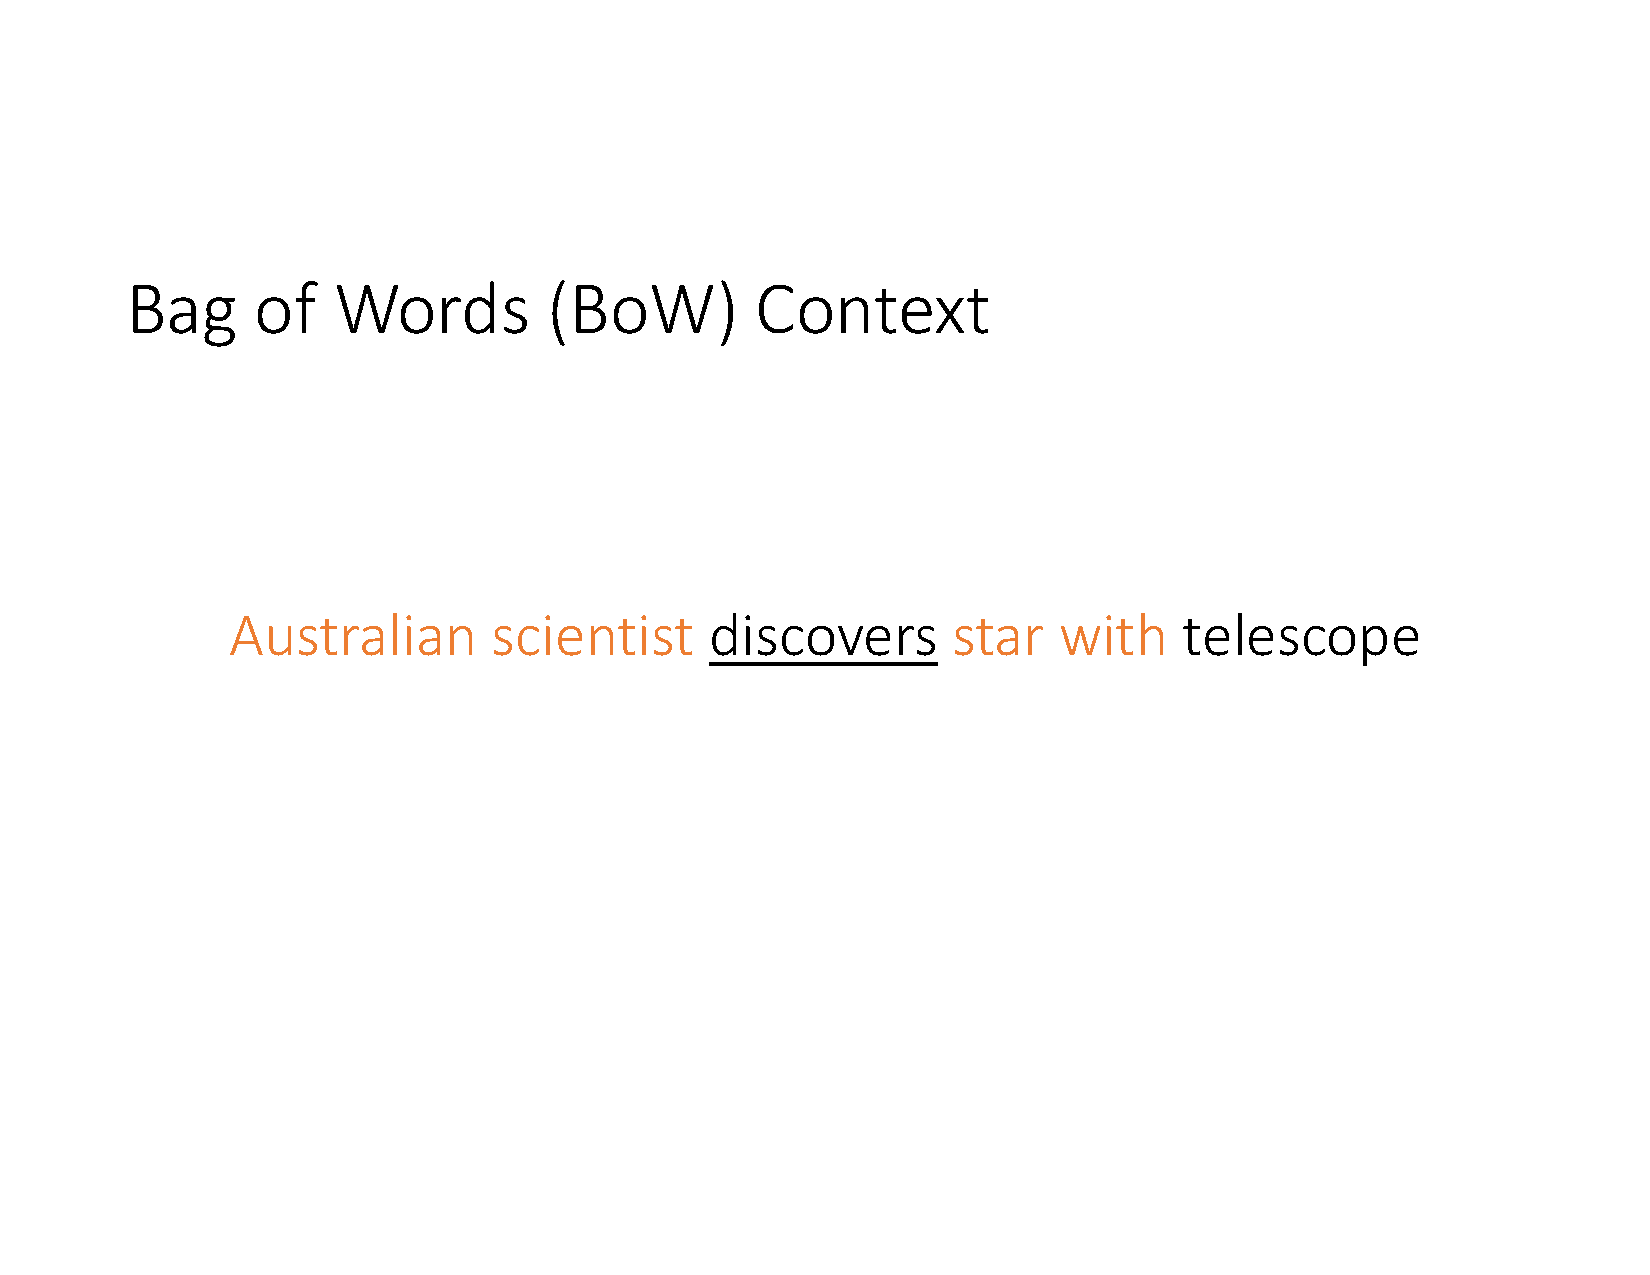
\includepdf[pages=-]{distsim/dep_embeddings.pdf}
}

\begin{frame}{Context matters}

    \begin{block}{Choose the correct contexts for your application}
        \begin{itemize}
            \item larger window sizes -- more topical
            \item dependency relations -- more functional
                \pause
            \item only noun-adjective relations
%                \scalebox{0.8}{
%                \begin{tabular}{cc}
%                    & \textbf{all dependencies} \\
%                            \hline
%                                   \textbf{sandwich}:
%                                   & satay, sandwiches, ravioli, doughnut, dessert, \\
%                                   & casserole, steak, shortbread, omelette, risotto \\
%                           \hline
%                           & \textbf{only noun-adj dependencies} \\
%                           \hline
%                                \textbf{sandwich}:
%                                & pizza, sandwiches, pan, pastry, doughnut \\
%                                & biscuit, doughnuts, burger, dessert, pies \\
%                            \end{tabular}}
%                \pause
            \item only verb-subject relations
                \pause
            \item context: time of the current message
            \item context: user who wrote the message
                \pause
            \item \ldots
            \item the sky is the limit
        \end{itemize}
    \end{block}

\end{frame}


\begin{frame}{Summary}
    \begin{block}{Distributional Semantics}
        \begin{itemize}
            \item Words in similar contexts have similar meanings.
            \item Represent a word by the contexts it appears in.
            \item But what is a context?
        \end{itemize}
    \end{block}
    \begin{block}{Neural Models (word2vec)}
        \begin{itemize}
            \item Represent each word as dense, low-dimensional vector.
            \item Same intuitions as in distributional vector-space models.
            \item Efficient to run, scales well, modest memory requirement.
            \item Dense vectors are convenient to work with.
            \item Still helpful to think of the context types.
        \end{itemize}
    \end{block}
\end{frame}


\end{document}

%%%% examples
